\documentclass{article}
\author{Shixiang (Adam) Yang}

\date{September 23, 2022}
\title{CSCI270 - Assignment3}
% \graphicspath{{./media/}}
\usepackage{algorithm}
\usepackage{algpseudocode}
\usepackage{tikz} 
\usepackage{amsfonts}
\usepackage{indentfirst}
\setlength\parindent{24pt}
\begin{document} \maketitle
\section{Problem 1}
\subsection{Problem a}
\subsubsection{Is the graph $(V,E')$ connected?}

With graph $(V,E)$ looks like the following:
\begin{center}
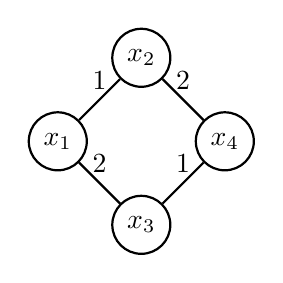
\begin{tikzpicture}[node distance={15mm}, thick, main/.style = {draw, circle}] 
\node[main] (1) {$x_1$}; 
\node[main] (2) [above right of=1] {$x_2$}; 
\node[main] (3) [below right of=1] {$x_3$}; 
\node[main] (4) [above right of=3] {$x_4$}; 
\draw (1) -- node[above] {1} (2); 
\draw (1) -- node[above] {2} (3); 
\draw (2) -- node[above] {2} (4); 
\draw (3) -- node[above] {1} (4);  
\end{tikzpicture}
\end{center}

 (V,E') will be disconnected because $E'$  only contains the cheapest edge for $x_1, x_2, x_3, x_4$. Therefore, the edges with weight of two are not contained in $E'$ because (1) for $x_1$, the edge $(x_1,x_3)$ is larger than $(x_1,x_2)$ (2) for $x_2$, the edge $(x_2,x_4)$ is larger than $(x_1,x_2)$ (3) for $x_3$, the edge $(x_1,x_3)$ is larger than $(x_3,x_4)$ (4) for $x_4$, the edge $(x_2,x_4)$ is larger than $(x_3,x_4)$. The graph $(V,E')$ looks like
\begin{center}
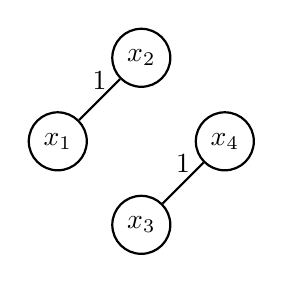
\begin{tikzpicture}[node distance={15mm}, thick, main/.style = {draw, circle}] 
\node[main] (1) {$x_1$}; 
\node[main] (2) [above right of=1] {$x_2$}; 
\node[main] (3) [below right of=1] {$x_3$}; 
\node[main] (4) [above right of=3] {$x_4$}; 
\draw (1) -- node[above] {1} (2); 
\draw (3) -- node[above] {1} (4);  
\end{tikzpicture}
\end{center}

Therefore, graph $(V,E')$ is not connected, proved by counterexample.

\subsubsection{Is the graph $(V,E')$ acyclic?}
Assume the graph has a cycle with $n$ edges and $n$ vertices, $\{v_1, v_2, ..., v_n\}$ [for every node $v_i$, it is connected to $v_{i-1}$ and $v_{i+1}$ for $i \in [1,n-1]$. $v_1$ is connected to $v_2$ and $v_n$, $v_n$ is connected to $v_{n-1}$ and $v_1$]. Consider this cycle $C$. Since the cost of every edge is distinct, there exists one largest edge. WLOG, look at a vertex $v_1 \in C$ and assume $c_{(v_1, v_2)}$ is largest. So, $c_{(v_1, v_2)} > c_{(v_1, v_n)}$, $c_{(v_1, v_2)} > c_{(v_2, v_3)}$. Since $E'$ only include the cheapest edge incident on $v_1, v_2$, $E'$ won't include $(v_1,v_2)$. Contradiction! QED. 




\subsection{Problem b}
\subsubsection{prove the output graph $(V,T)$ is a MST}
The output is a spanning tree. In each iteration, the algorithm combine at least two separate components $C_1, C_2$ into a larger connected component with an edge $e$. Therefore, a new element can be viewed as the combination of all vertices in $C_1, C_2$. Since the number of separate components will always decrease, the algorithm will always terminate when the number of connected components converges to 1, which is the combination of all vertices. Consider each component as a node, the algorithm can be viewed as finding the cheapest edge $e$ for each "contracted node". Proven above, this operation computes an acyclic graph. Thus, the output is a spanning tree because (1) it includes every vertex (2) it is a tree.

The output is a MST. WLOG, whenever an edge $e$ is added to a component $C$, it is explicitly chosen as the cheapest edge that connects $C$ and $\bar C$.   Therefore, each added edge is cheapest across some cut. By cut property, each cheapest edge is in MST. Thus, each newly created connected component after each iteration is a subset of MST. Since the output is always a spanning tree with $n-1$ edges, the output has to be a MST. Because $E$ is a connected graph, an edge can always be found or the algorithm terminates. QED

\subsubsection{prove that it can be done in $O(m\log{n})$}
Notice that for each separate component, it will be connected to at least one other connected components in each iteration. Therefore, with $i$ separate components at the beginning of the iteration, the algorithm produces at most $\frac{i}{2}$ new separate connected components. This happens when each new component only contains two previous components. 

The algorithm terminates when there are only two separate components at the start of an iteration. Let assume it take $k$ iterations until the algorithm terminates (only one component left in $(V,T)$ after $k$-th iteration).
\[\frac{n}{2^k}=1\]
Therefore, it takes $O(\log{n})$ iterations until $(V,T)$ is connected.

 To find cheapest edges for k components in each iteration, we can first have an array a[k] indexed from 1 to $k$, every element initialized to infinitely large integer. For $i\in[1,k]$, a[i] stores the cheapest edge for i-th component. Then, \textbf{For each edge in edges:}

1. check the component labels of its two endpoints

2. update a[ ] if the edge is cheaper\\
Since $(V,E)$ is a connected graph, $|E|\geq|V|-1 \rightarrow m\geq n-1$. Each iteration's running time is $O(m)$. Because there are $O(\log{n})$ iterations, each of which takes $O(m)$, the total running time is:
\[O(m)*O(\log{n})=O(m\log{n})\]


\section{Problem 2}
\subsection{Algorithm}
\begin{algorithm}
\textbf{Assumption:} the graph $(V,E)$ is connected, $\forall v \in V, \exists$ at least one solution
    \caption{An algorithm computing the earliest time that you can arrive at $d$ when starting at $s$ at time $T$}\label{alg:cap}
    \begin{algorithmic}
    \State Let $S$ be the set of explored nodes

    For each $u\in S$, we store an arrival time t(u)
    \State Initially $S = \{s\}$ and $d(s)$ = 0
    \While{$S\neq V$}

        \State Select a node $v\not\in S$ with at least one edge from S for which:
        \begin{enumerate}
            \item $\exists$ an edge $(u,v,t_u,t_v)$ with $u \in S$ and $t(u) \leq t_u$
            \item $v$ allows $t_v \leq$ any other arrival time for all the nodes $\not\in S$
        \end{enumerate}
        
        \State Add $v$ to $S$ and define $t(v) = t'(v)$
    \EndWhile
    \end{algorithmic}
    \end{algorithm}

In short, the algorithm greedily finds the earliest and time conflict-free node from the nodes that we have reached.

\subsection{Prove the correctness of algorithm}

We will show that every time the algorithm selects an edge to a vertex $v$, the arrival $t(v)$ is earlier than every other possible arrival time $t'(v)$ and there isn't any time conflict $\forall v\in S$. This fact can establish the correctness of the algorithm when we apply it to the end of the algorithm, when point $S$ includes all vertices. 

We prove this algorithm by induction on size of $S$.\\
\textbf{Claim:} Every time the algorithm selects an edge to a vertex $v$, the arrival time $t(v)$ no late than every other possible arrival time $t'(v)$ and there isn't any time conflict $\forall v\in S$.\\
\textbf{Base Case:} When $|S|=1$, we have $S=\{s\}$ and $t(s) = T+0 = T$. It is the earliest. No time conflict is trivial since only one node.\\
\textbf{Inductive Hypothesis:} Suppose the claim holds when $|S|=k$ for some value of $k \geq 1$; we now grow $S$ to size $k + 1$ by adding the node $v$. Let $(u, v, t_u, t_v)$ be the final edge on our $s-v$ path $P_v$.\\
\textbf{Inductive Step:} By induction hypothesis, $P_u$ is the earliest $s-u$ path for each $u\in S$ with no time conflict. Now consider any other $s-v$ path $P$; we wish to show that it is at least as long as $P_v$. In order to reach $v$, this path $P$ must leave the set $S$ somewhere; let $y$ be the first node on $P$ that is not in $S$, and let $x \in S$ be the node just before $y$.

Once $P$ leaves $S$ and reaches $y$, $P$ is at least as late as $P_v$ because the algorithm always explicitly picks the node that has the earliest arrival time among the node $\not\in S$: $t(v) \leq$ arrival time for all other nodes $\not\in S$. In the $k+1$ iteration, the algorithm must have considered adding node $y$ to the set $S$ via the edge $(x, y)$ and rejected this option in favor of adding $v$. This means that there is no path from $s$ to $y$ through $x$ that is shorter than $P_v$. But the sub-path of $P$ up to $y$ is such a path, and so this sub-path is at least as late as $P_v$. Since edge lengths are non-negative, the full path $P$ is at least as long as $P$, as well.

Notice that there can't be any time conflict because we only consider the point that the leaving time $t_u$ is no earlier than the u-node arriving time.

Thus, $P$ cannot be earlier than $P_v$. Claim is proved. QED.

\subsection{Prove the running time is $O(m\log{n})$}

\textbf{Implementation}:
\begin{algorithm}
\textbf{Assumption:} the graph $(V,E)$ is connected, $\forall v \in V, \exists$ at least one solution
    \begin{algorithmic}
    \State Let $S$ be the set of explored nodes
    \State Let $PQ$ be an empty priority queue, arrival time $t(v)$ as key, vertex $v$ as key
    \For {vertices $v_s \in V$}
        \If{$v == v_s$}
            \State $t(v_s) = 0$
        \Else
            \State $t(v) = \infty$
        \Endif
    \EndFor

    \State Initialize an empty set S to contain explored nodes
    \While{}
    \EndWhile
    \end{algorithmic}
    \end{algorithm}


We put the nodes $V$ in a priority queue with $t(v)$ as the key for $v \in V$, which takes $O(n\log{n})$. 
    1. changeKey for t(s) = T
    2. for loop through all the edges of the starting (for initialization t(v)) m * logn
    3. O(1), find
    4. extract logn degree to find the previous incident nodes in S
 

\end{document}
